\documentclass[12pt, titlepage]{article}

% All modules
% spaceShooter.py
% gameFunctions.py
% constants.py
% inGameAssets.py
% gameObjects.py
% __init__.py


\usepackage{fullpage}
\usepackage[round]{natbib}
\usepackage{multirow}
\usepackage{booktabs}
\usepackage{tabularx}
\usepackage{graphicx}
\usepackage{float}
\usepackage{hyperref}
\restylefloat{table}
\hypersetup{
    colorlinks,
    citecolor=black,
    filecolor=black,
    linkcolor=red,
    urlcolor=blue
}
\usepackage[round]{natbib}

\newcounter{acnum}
\newcommand{\actheacnum}{AC\theacnum}
\newcommand{\acref}[1]{AC\ref{#1}}

\newcounter{ucnum}
\newcommand{\uctheucnum}{UC\theucnum}
\newcommand{\uref}[1]{UC\ref{#1}}

\newcounter{mnum}
\newcommand{\mthemnum}{M\themnum}
\newcommand{\mref}[1]{M\ref{#1}}

\title{SE 3XA3: Module Guide\\SpaceShooter}

\author{Team \#105, SpaceShooter
		\\ Dananjay Prabaharan - prabahad
		\\ Nishanth Raveendran - raveendn
		\\ Hongzhao Tan - tanh10
}

\date{\today}



\begin{document}

\maketitle

\pagenumbering{roman}
\tableofcontents
\listoftables
\listoffigures

\begin{table}[H]
\caption{\bf Revision History}
\begin{tabularx}{\textwidth}{p{3cm}p{2cm}X}
\toprule {\bf Date} & {\bf Version} & {\bf Notes}\\
\midrule
March 13, 2020 & 1.0 & Initial Draft\\
\textcolor{red}{April 6, 2020} & \textcolor{red}{2.0} & \textcolor{red}{Rev1 Update - Updated overview section and fixed spelling errors within the document.}\\
\bottomrule
\end{tabularx}
\end{table}

\newpage

\pagenumbering{arabic}

\section{Introduction}

\subsection{Overview}
The SpaceShooter application is a recreation of the 1980s arcade game that enables users to shoot upcoming obstacles \textcolor{red}{(aliens and meteors)} with a spaceship. Users could temporarily upgrade their spaceships with power-ups while playing the game. \textcolor{red}{These power-ups include double shooting, shield, missile bullets, and etc. The primary goal of the game is to survive as long as possible.}

\subsection{Context}
The document that follows is the Module Guide of the SpaceShooter application. The purpose of the Module Guide is to demonstrate the deconstruction of the project and how each module serves its respective function/non-functional requirements. The primary intended audience for this document are the new project members, maintainers, and designers. The Module Guide is developed after outlining the requirements on the Software Requirements Specification (SRS). After completing the Module Guide, the next step within the design process is to construct the MIS of the SpaceShooter application. 

\subsection{Design Principles}
Following design principles are incredibly important to any software project to ensure great quality of code and maintainability. When decomposing SpaceShooter into its respective modules, the core design principles that are being followed are (1) encapsulation (2) information hiding and (3) low coupling and high cohesion. 

	
\subsection{Document Structure}
The remainder of the document is structured as follows:
\begin{itemize}

\item Section \ref{SecChange} provides the "Anticipated and Unlikely Changes" of the application.

\item Section \ref{SecMH} outlines the module deconstruction (Module Hierarchy) of the application.

\item Section \ref{SecConnection} outlines the connection between the requirements and modules of the application.

\item Section \ref{SecMD} provides the details of each module including its secrets and responsibilities. 

\item Section \ref{SecTM} provides 2 Traceability Matrices (1) Comparing the design completeness against the application's requirements (2) Connection between modules and anticipated changes.

\item Section \ref{SecUse} outlines the module's Uses Hierarchy for the application.
\end{itemize}	

\section{Anticipated and Unlikely Changes} \label{SecChange}

This section lists possible changes to the SpaceShooter system. There are anticipated changes which are listed in Section \ref{SecAchange}, and
unlikely changes are listed in Section \ref{SecUchange}.

\subsection{Anticipated Changes} \label{SecAchange}

\begin{description}
\item[\refstepcounter{acnum} \actheacnum \label{acOS}:] Program being kept up to date with any new operating systems.
\item[\refstepcounter{acnum} \actheacnum \label{acUI}:] The user interface and menu operations of the program.
\item[\refstepcounter{acnum} \actheacnum \label{acMobility}:] The player mobility options and controls. 
\item[\refstepcounter{acnum} \actheacnum \label{acEnemy}:] The addition of new enemy mobs.
\item[\refstepcounter{acnum} \actheacnum \label{acPowerSys}:] The power up system.
\item[\refstepcounter{acnum} \actheacnum \label{acPowerUps}:] The addition of new power ups.
\end{description}

\subsection{Unlikely Changes} \label{SecUchange}


\begin{description}
\item[\refstepcounter{ucnum} \uctheucnum \label{ucIO}:] Input/Output devices (Input: Keyboard, Output: Memory, Screen).
\item[\refstepcounter{ucnum} \uctheucnum \label{ucInput}:] There will always be
  a source of input data external to the software.
\item[\refstepcounter{ucnum} \uctheucnum \label{ucIO}:] The objective and core game play. 
\item[\refstepcounter{ucnum} \uctheucnum \label{ucIO}:] The score system. 
\item[\refstepcounter{ucnum} \uctheucnum \label{ucInput}:] The health and lives system. 
\item[\refstepcounter{ucnum} \uctheucnum \label{ucInput}:] The art style of all of the game objects. 
\end{description}

\section{Module Hierarchy} \label{SecMH}

\begin{table}[h!]
\centering
\begin{tabular}{p{0.3\textwidth} p{0.6\textwidth}}
\toprule
\textbf{Level 1} & \textbf{Level 2}\\
\midrule


{Hardware-Hiding Module} & \\
\midrule

\multirow{1}{0.3\textwidth}{Behaviour-Hiding Module} & Game State Module\\
& Game Functions Module \\
& Game Objects Module \\
\midrule

\multirow{1}{0.3\textwidth}{Software Decision Module} & Constants Module\\
& In-Game Assets Module \\
\bottomrule

\end{tabular}
\caption{Module Hierarchy}
\label{TblMH}
\end{table}

\begin{description}
\item [\refstepcounter{mnum} \mthemnum \label{mHH}:] Hardware-Hiding Module
\item [\refstepcounter{mnum} \mthemnum \label{mGS}:] Game State Module
\item [\refstepcounter{mnum} \mthemnum \label{mGF}:] Game Functions Module
\item [\refstepcounter{mnum} \mthemnum \label{mGO}:] Game Objects Module
\item [\refstepcounter{mnum} \mthemnum \label{mC}:] Constants Module
\item [\refstepcounter{mnum} \mthemnum \label{mIGA}:] In-Game Assets Module

\end{description}

\section{Connection Between Requirements and Design} \label{SecConnection}

The design of SpaceShooter is meant to satisfy the requirements established in the SRS. Each of the requirements are satisfied by a single or several module(s) with related information that are decomposed from the system. The Game State Module uses functionalities from all other modules but not the Hardware-Hiding Module to ensure the system can be correctly executed. The appearance, usability and game-state-related requirements are satisfied by Game State Module, image and audio files that are used in the implementation which provides a UI for users to operate the system and make correct respond on the UI due to requests from the users or state of the game.\newline
The system is written in Python which satisfies the requirement that the system shall be able to run on the mainstream operating systems. Maintainability requirements are satisfied by proper modularization and documentation in the implementation of the system. The connection between requirements and modules is listed in Table \ref{TblRT}.

\section{Module Decomposition} \label{SecMD}
\textcolor{red}{The  following  modules  are  decomposed  to  David  Parnas’  principle  of  information  hiding. They are broken down in the following matter, Secret, Service, and Implemented By. Secrets will describe in a single word what it is that the module is hiding. Services will detail what it is the module does, and Implemented By states by what means the module is implemented. However,  if  the  entry  is OS,  this  signifies  that  the  following  module  is  provided  by  the operating system.}
\subsection{Hardware Hiding Modules (\mref{mHH})}

\begin{description}
\item[Secrets:] The data structure and algorithms that supports the basic functionalities of users' hardware.
\item[Services:] Provides an interface between the hardware and \textcolor{red}{SpaceShooter}.
\item[Implemented By:] OS
\end{description}

\subsection{Behaviour-Hiding Module}

\subsubsection{Game State Module (\mref{mGS})}

\begin{description}
\item[Secrets:]The internal game data of the player and the game state. 
\item[Services:] Controls and updates the state of the game. This module will switch screens when the player pauses or dies. During the "Playing Game" state, this module will spawn meteors and aliens, checking if the player touches a meteor or power up, and update the game score, player health, and power up state. The module also invokes the game functions to draw the graphical output.  
\item[Implemented By:] gameState.py
\end{description}

\subsubsection{Game Function Module (\mref{mGF})}

\begin{description}
\item[Secrets:]The general functions that are used in the main running loop of the game.
\item[Services:]Generates main menu, pause menu and death menu when the game is in "Pre-Game State", and "Paused State" respectively; Displays the texts that are supposed to be shown on the UI with specified font and size; Displays the "shield bar" and "lives" which graphically acknowledge the user about the condition of the in-game spaceship when the system is in "Playing Game State"
\item[Implemented By:] gameFunctions.py
\end{description}

\subsubsection{Game Object Module (\mref{mGO})}

\begin{description}
\item[Secrets:]The respective properties and methods of each critical object in the game. 
\item[Services:]Defines the properties of each interactive object within the game (Missile, Bullet, Explosion, Player, etc); Establishes various object methods against different scenarios in the game.
\item[Implemented By:] gameObjects.py
\end{description}


\subsection{Software Decision Module}

\subsubsection{Constants Module (\mref{mC})}

\begin{description}
\item[Secrets:] The values of all constants that are used in the implementation
\item[Services:] Records the values of the width and height of the general UI screen, frame rate of the game, length and height of the UI for in-game spaceship's "shield bar", and the value of tuples which define colors of the general UI. 
\item[Implemented By:] constant.py
\end{description}

\subsubsection{In-Game Assets Module (\mref{mIGA})}

\begin{description}
\item[Secrets:] Data of each asset utilized in various stages of the game.
\item[Services:] Denotes the path to the assets being used in the game; Assigns and establishes which asset file to use for each object in the game.
\item[Implemented By:]InGameAssets.py
\end{description}

\section{Traceability Matrix} \label{SecTM}
% the table should use mref, the requirements should be named, use something
% like fref
\begin{table}[H]
\centering
\begin{tabular}{p{0.2\textwidth} p{0.6\textwidth}}
\toprule
\textbf{Req.} & \textbf{Modules}\\
R1 & \mref{mHH}\\
R2 & \mref{mGF}\\
R3 & \mref{mGF}\\
R4 & \mref{mGS}, \mref{mGF}\\
R5 & \mref{mGS}, \mref{mGF}\\
R6 & \mref{mGS}, \mref{mGF}\\
R7 & \mref{mGS}, \mref{mGF}\\
R8 & \mref{mGF}, \mref{mGO}\\
R9 & \mref{mGS}\\
R10 & \mref{mGO}\\
R11 & \mref{mGS}\\
R12 & \mref{mGS}\\
R13 & \mref{mGO}\\
R14 & \mref{mGO}\\
\textcolor{red}{R15} & \mref{mGS}, \mref{mGO}\\
\textcolor{red}{R16} & \mref{mGS}, \mref{mGO}\\
\textcolor{red}{R17} & \mref{mGS}, \mref{mGO}\\
\textcolor{red}{R18} & \mref{mGS}, \mref{mGO}\\
R19 & \mref{mGS}, \mref{mGF}, \mref{mGO}\\
\bottomrule
\end{tabular}
\caption{Trace Between Requirements and Modules}
\label{TblRT}
\end{table}

\begin{table}[H]
\centering
\begin{tabular}{p{0.2\textwidth} p{0.6\textwidth}}
\toprule
\textbf{AC} & \textbf{Modules}\\
\midrule
\acref{acOS} & \mref{mHH}\\
\acref{acUI} & \mref{mGF}\\
\acref{acMobility} & \mref{mGO}\\
\acref{acEnemy} & \mref{mGO}\\
\acref{acPowerSys} & \mref{mGS}\\
\acref{acPowerUps} & \mref{mGO}\\
\bottomrule
\end{tabular}
\caption{Trace Between Anticipated Changes and Modules}
\label{TblACT}
\end{table}

\section{Use Hierarchy Between Modules} \label{SecUse}

In this section, the uses hierarchy between modules is provided. For two modules A and B, A uses B means that it might be necessary for A to have access to a correct implementation of B, so that A can provide only desired functionalities to its clients.  Figure \ref{FigUH} illustrates the use relation between
the modules..

\begin{figure}[H]
\centering
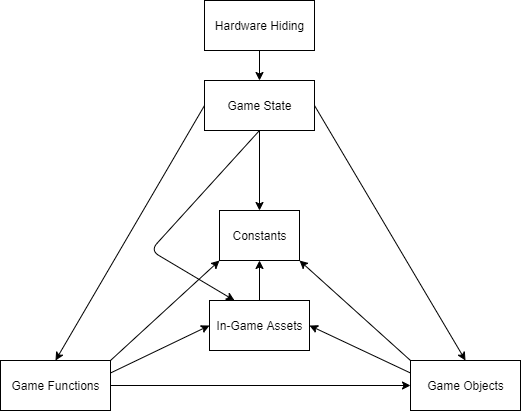
\includegraphics[width=0.7\textwidth]{UsesHierarchy.png}
\caption{Use hierarchy among modules}
\label{FigUH}
\end{figure}

\section{Gantt Chart}
\begin{figure}[H]
\centering
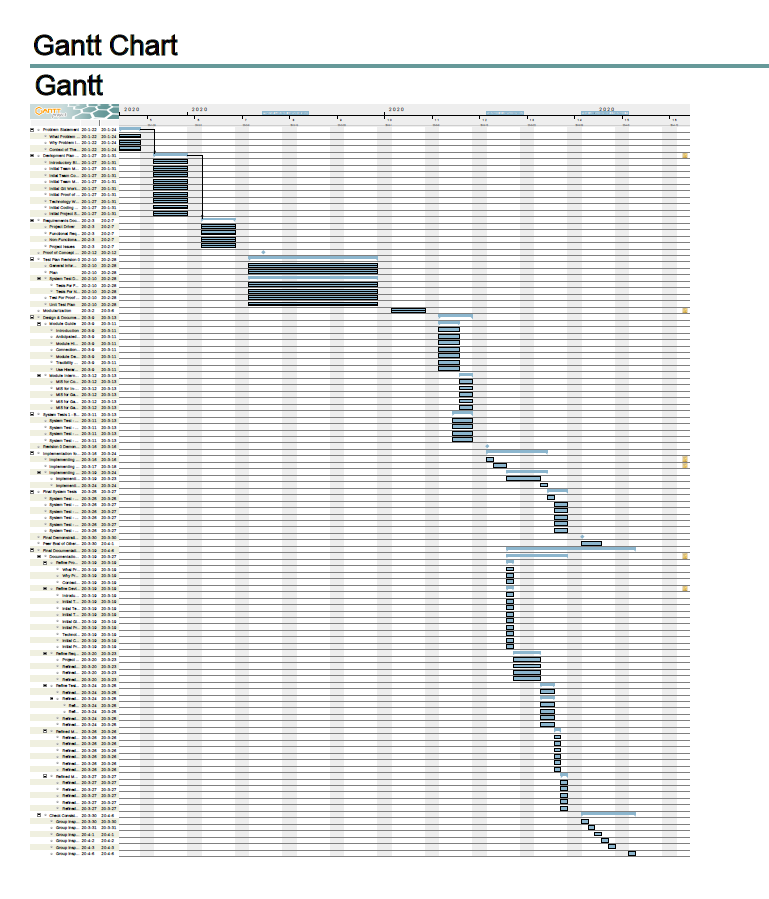
\includegraphics[width=0.95\textwidth]{GanttChartScreenShot.png}
\caption{Gantt Chart}
\label{FigUH}
\end{figure}


\end{document}